\documentclass[11pt]{report} % Tipo de documento

% Paquetes y configuraciones adicionales
\usepackage{graphicx}
\usepackage[export]{adjustbox}
\usepackage{caption}
\usepackage{float}
\usepackage{titlesec}
\usepackage{geometry}
\usepackage[hidelinks]{hyperref}
\usepackage{titling}
\usepackage{titlesec}
\usepackage{parskip}
\usepackage{wasysym}
\usepackage{tikzsymbols}
\usepackage[spanish]{babel}

% Configuración de los títulos de las secciones
\newcommand{\subtitle}[1]{
  \posttitle{
    \par\end{center}
    \begin{center}\large#1\end{center}
    \vskip0.5em}
}

% Configura los márgenes
\geometry{
    left=2cm,   % Ajusta este valor al margen izquierdo deseado
    right=2cm,  % Ajusta este valor al margen derecho deseado
    top=3cm,
    bottom=3cm,
}

% Configuración de los títulos de las secciones
\titlespacing{\section}{0pt}{\parskip}{\parskip}
\titlespacing{\subsection}{0pt}{\parskip}{\parskip}
\titlespacing{\subsubsection}{0pt}{\parskip}{\parskip}

% Redefinir el formato de los capítulos y añadir un punto después del número
\makeatletter
\renewcommand{\@makechapterhead}[1]{%
  \vspace*{0\p@} % Ajusta este valor para el espaciado deseado antes del título del capítulo
  {\parindent \z@ \raggedright \normalfont
    \ifnum \c@secnumdepth >\m@ne
        \huge\bfseries \thechapter.\ % Añade un punto después del número
    \fi
    \interlinepenalty\@M
    #1\par\nobreak
    \vspace{10pt} % Ajusta este valor para el espacio deseado después del título del capítulo
  }}
\makeatother

% Configura para que cada \chapter no comience en una pagina nueva
\makeatletter
\renewcommand\chapter{\@startsection{chapter}{0}{\z@}%
    {-3.5ex \@plus -1ex \@minus -.2ex}%
    {2.3ex \@plus.2ex}%
    {\normalfont\Large\bfseries}}
\makeatother

\begin{document}

% Portada del informe
\title{Practicaa 08. Configurando un Firewall con DMZ}
\subtitle{Seguridad de Sistemas Informáticos}
\author{Cheuk Kelly Ng Pante (alu0101364544@ull.edu.es)}
\date{\today}

\maketitle

% Índice
\tableofcontents

% Nueva página 
\cleardoublepage

% Secciones del informe
% Capitulo 1
\chapter{Configuración de red con un sólo firewall, zona privada y DMZ}
Para esta primera parte se crean primero las tres máquina en el IAAS y se configuran las diferentes interfaces de red 
de cada una de ellas. Para ello, se accede al fichero \emph{/etc/network/interfaces} y se configuran las siguientes redes 
siguiendo el siguiente direccionamiento:
\begin{itemize}
  \item \textbf{Internet:} red especificada por el servidor DHCP externo
  \item \textbf{Red Interna:} red de clase C privada como subred de una clase B privada: 172.16.10.0/24
  \item \textbf{DMZ:} red de clase C privada 192.168.10.0/24
\end{itemize}

\begin{figure}[H]
  \centering
  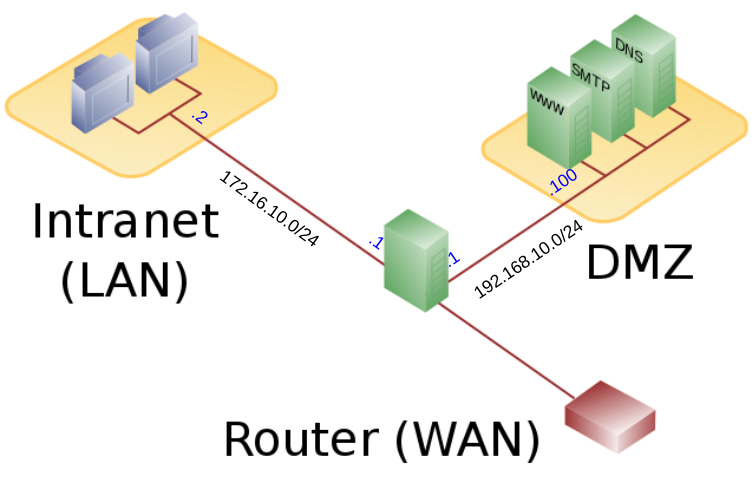
\includegraphics[scale=0.4]{img/esquema_red.png}
  \caption{Esquema de red}
  \label{fig:esquema de red}
\end{figure}

La configuración de red de cada máquina se muestra a continuación:
\begin{itemize}
  \item Maquina 1: \emph{Firewall}
  \begin{verbatim}
# The primary network interface
allow-hotplug ens3
iface ens3 inet dhcp

# The second network interace -> Server
auto ens4
iface ens4 inet static
        address 192.168.10.1
        netmask 255.255.255.0

# The third network interface -> Client
auto ens7
iface ens7 inet static
        address 172.16.10.1
        netmask 255.255.255.0
  \end{verbatim}

  \item Maquina 2: \emph{Cliente}
  \begin{verbatim}
# The second network interface
auto ens4
iface ens4 inet static
    address 172.16.10.2
    netmask 255.255.255.255
    gateway 172.16.10.1
  \end{verbatim}
\end{itemize}

Para las diferentes máquinas, a excepción del firewall, hay que deshabilitar la interfaz de la red publica. Para ello, en el mismo fichero de configuración
de las interfaces red, se borra la configuración de la interfaz que sea de la red pública y se reinicia los servicios de red.

% Nueva página 
\cleardoublepage

% Capitulo 2
\chapter{Configuracion de la red interna y un servidor en la DMZ}
Para este apartado se configura la red interna y se instala un servidor web en la DMZ. 
Primero debemos instalar en el cliente un navegor web, en este caso se instala \emph{links} 
con el comando \emph{sudo apt-get install links}. Luego, instalamos en la maquina servidor, el servidor web \emph{nginx}
con el comando \emph{sudo apt-get install nginx}. 

Antes de realizar la configuración de \emph{nginx}, se debe configurar la red DMZ, del servidor web. Para ello, se accede al fichero
\emph{/etc/network/interfaces} y asignamos la IP privada 192.168.10.100/24 y como gateway la IP privada del firewall, entonces el fichero
de configuración de la red DMZ añadimos lo siguiente:
\begin{verbatim}
# The second network interface
auto ens4
iface ens4 inet static
      address 192.168.10.100
      netmask 255.255.255.0
      gateway 192.168.10.1
\end{verbatim}

Ya configurado la red DMZ, se procede a configurar el servidor web. Para ello, se accede al fichero \\
\emph{/etc/nginx/sites-available/default} y se modifica el fichero de la siguiente manera:

\begin{verbatim}
server {
  listen 192.168.10.100:80;
  server_name 10.6.129.251;
}
\end{verbatim}

Una vez modificado el fichero, se reinicia el servidor web con el comando \emph{sudo systemctl restart nginx}.

\begin{figure}[H]
  \centering
  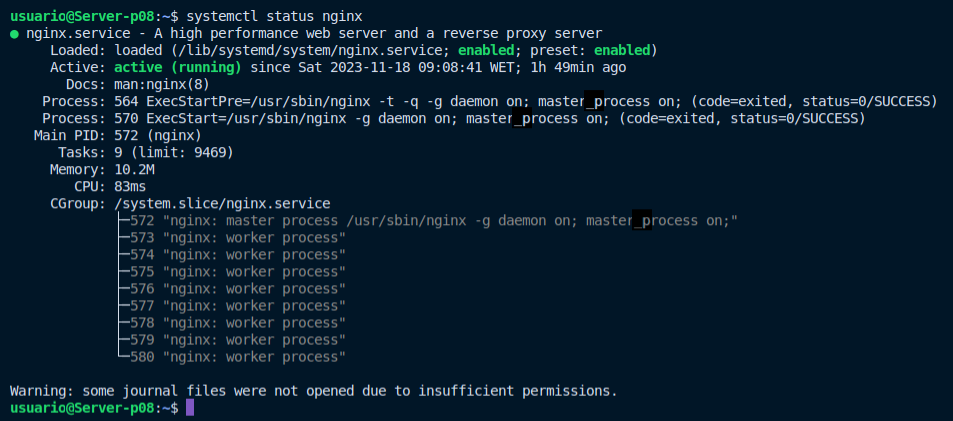
\includegraphics[scale=0.4]{img/nginx_status.png}
  \caption{Estado del servidor web nginx}
  \label{fig:estado del servidor web nginx}
\end{figure}

% Nueva página
\cleardoublepage

% Capitulo 3
\chapter{Reglas de filtrado para el firewall}
El script de configuración del firewall se muestra a continuación:

\begin{verbatim}
#!/bin/bash

# Reset de las reglas
iptables -P INPUT DROP
iptables -P FORWARD DROP
iptables -P OUTPUT ACCEPT
iptables -F
iptables -X
iptables -Z
iptables -t nat -F
iptables -t nat -X
iptables -t nat -Z

# Acceso ssh al firewall
iptables -A INPUT -m state --state RELATED,ESTABLISHED -j ACCEPT
iptables -A INPUT -i ens3 -p tcp --dport 22 -j ACCEPT

# Acceder desde la red interna (con la ip publica) a los servicios web
iptables -t nat -A PREROUTING -i ens3 -p tcp --match multiport 
--dports 80,443 -j DNAT --to 192.168.10.100:80 
iptables -t nat -A PREROUTING -i ens4 -d 10.6.129.251 -p tcp --match multiport 
--dports 80,443 -j DNAT --to-destination 192.168.10.100:80 

# Acceder desde la red interna a servidores Web de Internet
iptables -A FORWARD -i ens4 -p tcp --match multiport --dports 80,443 -j ACCEPT
iptables -A FORWARD -i ens7 -p tcp --match multiport --dports 80,443 -j ACCEPT

# Permite acceder a los servicios web (DMZ) desde internet
iptables -A FORWARD --match state --state ESTABLISHED,RELATED -j ACCEPT
iptables -A FORWARD -i ens3 -o ens7 -p tcp --match multiport --dports 80,443 -j ACCEPT

# Permitir tráfico DNS
iptables -A FORWARD -p udp --dport 53 -j ACCEPT
iptables -A FORWARD -p udp --dport 53 -j ACCEPT

iptables -t nat -A POSTROUTING -o ens3 -j MASQUERADE
\end{verbatim}

% Nueva página
\cleardoublepage

Para permitir tráfico web desde la red interna a los servidores web de Internet, se debe añadir las siguientes reglas:
\begin{verbatim}
iptables -A FORWARD -i ens4 -p tcp --match multiport --dports 80,443 -j ACCEPT
iptables -A FORWARD -i ens7 -p tcp --match multiport --dports 80,443 -j ACCEPT
\end{verbatim}

\begin{figure}[H]
  \centering
  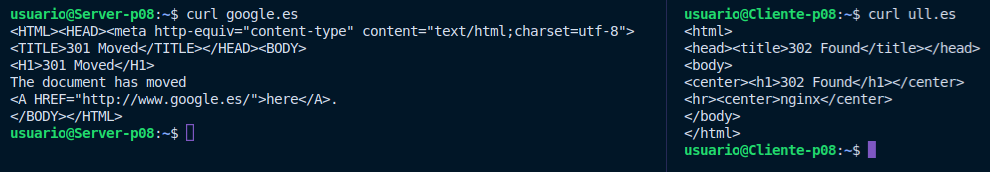
\includegraphics[scale=0.4]{img/web_internet.png}
  \caption{Accediendo a los servidores web de Internet desde la red interna}
  \label{fig:permitir tráfico web desde la red interna a los servidores web de Internet}
\end{figure}

Para permitir el tráfico Web desde Internet al servidor web que se encuentra en la DMZ, se debe añadir las siguientes reglas:
\begin{verbatim}
iptables -A FORWARD --match state --state ESTABLISHED,RELATED -j ACCEPT
iptables -A FORWARD -i ens3 -o ens7 -p tcp --match multiport --dports 80,443 -j ACCEPT
\end{verbatim}

\begin{figure}[H]
  \centering
  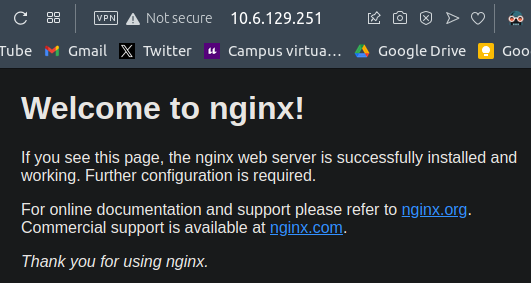
\includegraphics[scale=0.55]{img/nginx_navegador.png}
  \caption{Accediendo al servidor web de la DMZ desde Internet}
  \label{fig:permitir tráfico web desde Internet al servidor web que se encuentra en la DMZ}
\end{figure}

Y por último, para permitir el tráfico Web desde la red interna al servidor web de la DMZ, se debe añadir las siguientes reglas:
\begin{verbatim}
iptables -t nat -A PREROUTING -i ens3 -p tcp --match multiport 
--dports 80,443 -j DNAT --to 192.168.10.100:80 
iptables -t nat -A PREROUTING -i ens4 -d 10.6.129.251 -p tcp --match multiport 
--dports 80,443 -j DNAT --to-destination 192.168.10.100:80 
\end{verbatim}

% Nueva página
\cleardoublepage

En la siguiente figura se muestra el acceso al servidor web de la DMZ desde la red interna.

\begin{figure}[H]
  \centering
  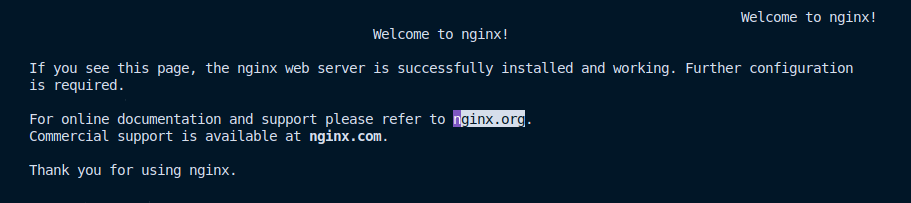
\includegraphics[scale=0.5]{img/nginx_cliente.png}
  \caption{Accediendo al servidor web de la DMZ desde la red interna}
  \label{fig:permitir tráfico web desde la red interna al servidor web de la DMZ}
\end{figure}

\end{document}